\chapter{Ejercicio Sigue Personas simulado en Robotics Academy}
\label{cap:capitulo5}

En este capítulo se presenta la elaboración del ejercicio Follow Person para Robotics Academy empezando desde el desarrollo interno de la infraestructura del ejercicio hasta una solución óptima que realice la tarea de seguir a una persona.



% -- SECCION ENTORNO GAZEBO
% ---------------------------
\section{Entorno simulado de un hospital}
\label{sec:hospital_gazebo}

La primera tarea fue integrar un entorno para Gazebo sobre el cual el robot Turtlebot2 tendría que enfrentarse. El entorno candidato que elegimos fue un \textbf{Hospital} debido a las siguientes ventajas:

\begin{enumerate}
	\item El robot se enfrenta a un entorno complejo (paredes, obstáculos, varias personas).
	\item La tarea Sigue Personas tendría lugar en un entorno en el cuál tiene sentido verlo en el mundo real. Los Robots en el ámbito de la salud están en continua integración.
\end{enumerate}

De modo que incorporamos el siguiente mundo de Gazebo que proporciona AWS (Amazon Web Service) en uno de sus repositorios de Github \footnote{\url{https://github.com/aws-robotics/aws-robomaker-hospital-world}}:

\begin{figure} [H]
  \begin{center}
    \includegraphics[width=10cm]{imagenes/hospital_world.png}
  \end{center}
  \caption[Hospital de AWS en Gazebo]{Hospital de AWS en Gazebo}
  \label{fig:hospital_gazebo}
\end{figure}

El repositorio proporcionaba varios ficheros \textbf{.world} con distintas versiones del Hospital: solo planta baja, una planta y dos plantas. Elegimos por comodidad la primera.\\

El siguiente paso era integrar una persona que pudiera desplazarse por el entorno.



% -- SECCION TELEOPERADOR
% -------------------------
\section{Teleoperador}
\label{sec:teleoperador}

El objetivo final es que el usuario que use la plantilla web pueda mover manualmente una persona del Hospital para que el robot pueda seguirla. Para ello teníamos que desarrollar un teleoperador.\\

El primer punto de partida era integrar una persona en el nuevo entorno simulado, por lo que accedimos a este repositorio \footnote{\url{https://github.com/osrf/gazebo_models}} que incorpora una librería de modelos para Gazebo e insertamos en el repositorio de Robotics Academy de terceros \textbf{Custom Robots} el modelo \textbf{\textit{person standing}}

\begin{figure} [H]
  \begin{center}
    \includegraphics[width=10cm]{imagenes/person_model.png}
  \end{center}
  \caption[Persona simulada en Gazebo]{Persona simulada en Gazebo}
  \label{fig:persona_gazebo}
\end{figure}

Ahora bien, el modelo es estático, carece de capacidad de desplazamiento, por lo que fue necesario desarrollar un plugin para Gazebo que permitiera ser controlado o que pueda desplazarse a través de una ruta que eligiera el programador. De modo que en el mismo paquete donde tenía los ficheros de lanzamiento del hospital diseñe el plugin (escrito en C++) al que denominé \textbf{libpersonplugin.so} para incorporarlo en el fichero \textbf{.sdf} (similar a URDF) de la persona. En este enlace podréis ver el \textbf{código fuente}\footnote{\url{https://github.com/JdeRobot/CustomRobots/blob/foxy-devel/amazon_hospital/hospital_world/src/person.cpp}}\\

El plugin requiere \textbf{2 funcionalidades}:
\begin{enumerate}
	\item \textbf{Comunicación remota} para el control manual. La intención es que el usuario se comunique con el modelo simulado, por lo tanto diseñé un \textbf{socket} de comunicaciones para dicha tarea.
	\item \textbf{Establecimiento de una ruta} por defecto y capacidad de incorporar nuevas rutas. Esta última funcionalidad no es necesaria para el ejercicio, además de que puede suponer cierta molestia al usuario, pero no se descarta su utilidad para un futuro.
\end{enumerate}

% -- SUBSECCION COMUNICACION REMOTA
% ----------------------------------
\subsection{Comunicación remota}
\label{subsec:comunicacion_remota}

En el propio fichero \textbf{person.cpp} creé 2 hilos (threads). Uno actuaría como servidor de un socket de comunicaciones que usaría el protocolo de transporte \textbf{UDP} (No esta orientado a la conexión y es más rápido). Dentro del socket implementé un protocolo de comunicación que entendierá el servidor, el cual sería únicamente receptor de los mensajes del cliente. Los mensajes que puede recibir son:

\begin{itemize}
	\item \textbf{``UVF"} (User Velocity Forward). El modelo se mueve hacia delante.
	\item \textbf{``UVB"} (User Velocity Backward). El modelo se mueva hacia atrás.
	\item \textbf{``UAR"} (User Angular Right). El modelo gira hacia la derecha.
	\item \textbf{``UAL"} (User Angular Left). El modelo gira hacia la izquiera.
	\item \textbf{``US-"} (User Stop). El modelo se detiene.
	\item \textbf{``A--"} (Autonomous). El modelo pasa a modo autónomo. Sigue la ruta establecida (actualmente desactivada).
\end{itemize}

Pero ¿dónde entra en juego el cliente? El fichero \textbf{exercise.py} incorpora un socket de comunicación UDP que se conecta al servidor del plugin a través del puerto 36677. Además, el \textbf{exercise.py} es el servidor de un WebSocket en comunicación con la plantilla web. Cuando el usuario haga click en el botón ``Teleoperate", el fichero de eventos de Javascript podrá enviar a través de un Websocket, que usa el puerto 1905, las teclas pulsadas para que el exercise.py se lo retransmita al plugin. Al iguál que en la comunicación \textbf{plugin-exercise.py}, implementé un protocolo de comunicación para \textbf{exercise.py-exercise.html}. Los mensajes que puede recibir son:

\begin{itemize}
	\item \textbf{``\#teleop\_true"}. Activa la teleoperación. A partir de ese momento, el usuario puede pulsar los botones ``awsdx". Envía un mensaje \textbf{``US-"} al plugin.
	\item \textbf{``\#teleop\_false"}. Desactiva la teleoperación. Pasa a modo autónomo (si estuviera activado). Envía una mensaje \textbf{``A--"} al plugin.
	\item \textbf{``\#key\_a"}. Envía un mensaje \textbf{``UAR"} al plugin.
	\item \textbf{``\#key\_d"}. Envía un mensaje \textbf{``UAL"} al plugin.
	\item \textbf{``\#key\_w"}. Envía un mensaje \textbf{``UVF"} al plugin.
	\item \textbf{``\#key\_s"}. Envía un mensaje \textbf{``UVB"} al plugin.
	\item \textbf{``\#key\_x"}. Envía un mensaje \textbf{``US-"} al plugin.
\end{itemize}

A continuación podemos ver un esquema que resuma la comunicación existente entre el exercise.html (incorpora el fichero ws\_code.js) con el plugin:

\begin{figure} [H]
  \begin{center}
    \includegraphics[width=15cm]{imagenes/comunicacion-teleoperador.png}
  \end{center}
  \caption[Comunicación del teleoperador]{Comunicación del teleoperador}
  \label{fig:comunicacion_teleoperador}
\end{figure}

% -- SUBSECCION DESPLAZAMIENTO DEL MODELO
% -----------------------------------------
\subsection{Desplazamiento del modelo}
\label{subsec:desplazamiento_modelo}




% -- SECCION HAL
% ----------------
\section{Desarrollo de la Capa de Abstracción Hardware (HAL)}
\label{sec:turtlebot2_hal_simulado}

\begin{figure} [H]
  \begin{center}
    \includegraphics[width=15cm]{imagenes/vista-planta-turtlebot2.png}
  \end{center}
  \caption[Láser Turtlebot 2]{Láser Turtlebot 2}
  \label{fig:vista_planta_turtlebot2}
\end{figure}
(TODO)




% -- SECCION SIGUE PERSONAS
\section{Solución Sigue-Personas Simulado}
\label{sec:sigue_personas_simulado}

En esta sección explicaremos la elaboración de una solución óptima del problema Sigue Personas para este ejercicio en simulado. Para ello, abarcaremos varios objetivos:
